\documentclass[conference]{IEEEtran}
\IEEEoverridecommandlockouts
% The preceding line is only needed to identify funding in the first footnote. If that is unneeded, please comment it out.
\usepackage{cite}
\usepackage{amsmath,amssymb,amsfonts}
\usepackage{algorithmic}
\usepackage{graphicx}
\usepackage{textcomp}
\usepackage{xcolor}
\usepackage{url} 
\usepackage{listings}
\usepackage{blindtext}
\usepackage[most]{tcolorbox}

\makeatletter
\NewDocumentCommand{\mynote}{+O{}+m}{%
  \begingroup
  \tcbset{%
    noteshift/.store in=\mynote@shift,
    noteshift=1.5cm
  }
  \begin{tcolorbox}[nobeforeafter,
    enhanced,
    sharp corners,
    toprule=1pt,
    bottomrule=1pt,
    leftrule=0pt,
    rightrule=0pt,
    colback=yellow!20,
    #1,
    left skip=\mynote@shift,
    right skip=\mynote@shift,
    overlay={\node[right] (mynotenode) at ([xshift=-\mynote@shift]frame.west) {\textbf{Note:}} ;},
    ]
    #2
  \end{tcolorbox}
  \endgroup
  }
\makeatother

\def\BibTeX{{\rm B\kern-.05em{\sc i\kern-.025em b}\kern-.08em
    T\kern-.1667em\lower.7ex\hbox{E}\kern-.125emX}}

\usepackage{xcolor}

\definecolor{codegreen}{rgb}{0,0.6,0}
\definecolor{codegray}{rgb}{0.5,0.5,0.5}
\definecolor{codepurple}{rgb}{0.58,0,0.82}
\definecolor{backcolour}{rgb}{0.95,0.95,0.92}

\lstdefinestyle{mystyle}{
    backgroundcolor=\color{backcolour},   
    commentstyle=\color{codegreen},
    keywordstyle=\color{magenta},
    numberstyle=\tiny\color{codegray},
    stringstyle=\color{codepurple},
    basicstyle=\ttfamily\footnotesize,
    breakatwhitespace=false,         
    breaklines=true,                 
    captionpos=b,                    
    keepspaces=true,                 
    numbers=left,                    
    numbersep=5pt,                  
    showspaces=false,                
    showstringspaces=false,
    showtabs=false,                  
    tabsize=2
}

\lstset{style=mystyle}

    
\begin{document}

\title{CS598 CCC Milestone 4\\
}

\author{
\IEEEauthorblockN{Cameron Greenwalt}
\IEEEauthorblockA{
\textit{UIUC}\\
Champaign, IL, USA \\
cg50@illinois.edu}
\and
\IEEEauthorblockN{Ming Meng}
\IEEEauthorblockA{
\textit{UIUC}\\
Champaign, IL, USA \\
mingm4@illinois.edu}
\and
\IEEEauthorblockN{Yang Peng}
\IEEEauthorblockA{
\textit{UIUC}\\
Champaign, IL, USA \\
yangp3@illinois.edu}
}
\maketitle


\section{Introduction} \label{sec:introduction}

Artificial Intelligence for IT Operations (AIOps) is the field in which AI methods are used to solve common IT problems. Use of AIOps in organizations of all sizes is appealing because AIOps has the potential to accelerate the resolution process of IT problems. The cloud computing field is prone to incidents that require IT expertise and resources to resolve, as applications deployed onto cloud systems are often complex. In the event that an incident occurs in an organization's cloud application, the site reliability engineers (SREs) tasked with resolving the incident are likely to encounter difficulty in diagnosing a root cause for the cloud application's faulty state. \cite{chen2020aiops} \cite{mani2023enhancing}

In the process of diagnosing a cloud incident's root cause, the SREs will analyze logs from applications and services involved in the incident. The objective in analyzing cloud logs is to assess application state, determine the inputs that led to that state, and trace what other services could have been affected by that state. The task of analyzing logs is arduous and slow because logs often are verbose, difficult to parse, numerous, and not human-reader friendly. If AI can be used to effectively accelerate this process of log analysis, then SREs can diagnose incidents more efficiently and businesses can expect to reduce costs and increase profits. \cite{10212414} \cite{gupta2023learning} Cloud system downtime creates dissatisfied customers and wasteful overhead as compute resources are provisioned but not used to generate revenue. \cite{li2022an} Reducing the amount of time required for SREs to diagnose cloud incidents will lead to shorter and less frequent cloud application downtime, which in turn leads to greater revenue generation.

However, the application of AI methods to solve IT problems is often expensive. \cite{LEE2023110689} \cite{network-log-anomaly-detection} AI solutions often necessitate teams of machine learning experts that know how to train, deploy, and maintain AI models. \cite{aiops-challenges} AI model training can be prohibitively expensive--even in cases where models are fine-tuned using domain-specific data rather than trained from scratch. Any AI model that can be deployed and provide acceptable use-case performance without a prerequisite training step on domain-specific data is preferable to a model that does require such training. Therefore, we would like to minimize the amount of training and fine-tuning required to use an AI model to analyze logs. We plan to do this by utilizing existing pre-trained large language models (LLMs).

In this research, we aim to accelerate the rate at which SREs can analyze logs by using natural language processing (NLP) LLMs to summarize cloud application logs, thus providing SREs with shorter and more easily understood and parsed representations of logs, which representations will retain the critical information contained within the original logs. \cite{medium-text-summarization} Specifically, we will use the ChatGPT family of LLMs to generate the log summaries. We plan to boost the the quality of generated log summaries by providing ChatGPT with additional contextual understanding of log semantics by embedding domain-specific text with the ADA embedding model and using the resultant embedding vectors as additional input to ChatGPT. We hypothesize that doing so will improve model performance in a particular domain (e.g., logs belonging to one type of application such as Apache Zookeeper) without requiring prior training or fine-tuning steps. In other words, the ChatGPT model parameters will remain unchanged.

Our solution will be a cloud-based, chat-oriented application hosted on Microsoft's Azure cloud hosting platform. The application will use the Azure OpenAI Service API to perform text embedding and ChatGPT inference steps.

We evaluate the quality of the generated log summaries by summarizing logs from Apache Zookeeper \cite{zookeeper} calculating several NLP text generation evaluation metrics on the generated summaries. In previous milestones, we had said we would logs from the Proxifier \cite{proxifier} application, but we have since pivoted to using Zookeeper logs because they are more diverse and information-rich than Proxifier logs. The metrics for evalutation that we compute include ROUGE \cite{lin2004rouge}, BERTScore \cite{bert-score}, BLEURT \cite{sellam2020bleurt}, BLEU \cite{10.3115/1073083.1073135}, NUBIA \cite{kane2020nubia}, and METEOR \cite{banerjee-lavie-2005-meteor}. Additionally, we perform log summarization using other baseline methods and assess the effectiveness of our proposed solution to that of the baseline methods by comparing the values of the previously listed metrics for both our solution and the baseline methods.

The summary of our major contributions is as follows:

\begin{itemize}
    \item We implement a novel method for summarizing cloud application logs using the ChatGPT family of generative models.
    \item We provide ChatGPT with deeper understanding of cloud application logs by embedding domain/application-specific text using the ADA embedding model and using the resulting vector embeddings to provide additional prompt input to ChatGPT.
    \item Our solution is a chat-based approach to generating log summaries. Chat-based approaches are accessible for experts and non-experts alike and can be adapted to be more scalable and automated.
\end{itemize}

\section{Prior work}

Many prior research works have addressed the topic of log summarization. LogSummary \cite{10017337} is perhaps the work in closest relation to what we would like to accomplish in our research. LogSummary is an automatic and unsupervised log summarization framework that achieves an impressive ROUGE F1 score. The authors, upon finding that no"gold standard" labelled dataset of logs and their associated summaries exists, created their own dataset of logs and log summaries. They used this dataset to assess the quality of their models. We will use their open-source dataset in our work to assess the quality of our methods.

At the core of LogSummary is the LogIE algorithm, which "performs open information extraction on logs, extracting triples relating entities and arguments through relation or predicate." \cite{10017337} Listing \ref{lst:zookeeper-summary} shows an example summary from LogSummary of the Zookeeper log shown in Listing \ref{lst:zookeeper-example}. LogSummary does \textit{not} use generative LLMs such as ChatGPT, BERT, or derivatives. Rather, it uses a rule-based approach to extract information from logs. We plan to use LLMs to accomplish a similar objective while not being constrained to this research work's entities-events-relation triple output summary format or including complicated logic.

\begin{figure}[h]
\begin{lstlisting}[numbers=none, caption=LogSummary Zookeeper Summary, label={lst:zookeeper-summary}]
 Accepted socket connection;Connection request will be dropped; Client attempting to establish new session; Established session timeout;
\end{lstlisting}
\end{figure} 

Some authors acknowledge that the ChatGPT model is more accurate than many other open source models that are presently available for summary generation. Additionally, ChatGPT often generates acceptable results without requiring a fine-tuning step prior to running inference. Presently, ChatGPT is the gold standard for most generative NLP tasks.\cite{bendimerad2023onpremise}

LogRule \cite{logrule} is a Root Cause Analysis (RCA) algorithm that offers a time-efficient, accurate, and interpretable solution for RCA in complex datasets--especially where the current state-of-the-art algorithm struggles with execution times. LogRule aims to provide an explanation for specific events of interest, but it depends on structured rather than unstructured logs, which means that doing log preprocessing or overhauling a system's logs to all be structured are prerequisites to using the system.

CloudRCA is "a root cause analysis framework for Alibaba Cloud's big data cloud computing platforms, utilizing heterogeneous multi-source data, state-of-the-art anomaly detection, and log analysis techniques to extract features, which are then employed in a Knowledge-informed Hierarchical Bayesian Network (KHBN) model." \cite{10.1145/3459637.3481903} CloudRCA is a thorough, useful system that is in-use in Alibaba's cloud systems. The authors claim that CloudRCA has provided a 20\% time savings for site reliability engineers (SREs). The cost for an organization to implement CloudRCA or a similar system in their own cloud platforms may exceed its relative benefit as it is quite niche and may not be generally applicable to dissimilar use cases. We envision that our work will have more general applicability and lower implementation cost for various organizations at the expense of narrower scope of operations, focusing on only the log summarization step of the incident analysis pipeline.

In \cite{10172904}, researchers showed that LLMs are effective in both identifying an incident's root cause and suggesting mitigation steps for the incident. This gives us confidence to proceed in our ChatGPT-based log summarization research.

BERT is a popular LLM alternative to ChatGPT that is used in cloud log-related tasks. BERT can be successful in performing specific tasks such as detection and classification but suffers from a lack of generalizability to different problem scopes. In addition, tasks using BERT and its derivatives often require training and fine-tuning steps. We have discussed previously that we do not want to perform any pre-training steps to obtain a useful model.

The performance of the anomaly log detection task using fine-tuned BERT-based models has proven to be very successful in recent research. For example, in one study, researchers were able to achieve an F1 score above 0.9 in detecting anomalies in a sample HDFS log dataset. This success can be attributed to the fact that HDFS log data is more structured than unstructured. In fact, the authors found that pre-training BERT with more natural language data had a negative impact on anomaly detection. \cite{LEE2023110689} From these researchers' experience, we hypothesize that ChatGPT may be better suited for logs with more natural language semantics.

In another study, the authors used the RoBERTa, a BERT derivative. The authors fine-tuned their model on both external and internal datasets, often borrowing popular new websites and articles. \cite{saha2022mining}

Another team of researchers used BERT-based models to build an intelligent-based system for IT Incident Operations. However, the metric scores they achieved with the base BERT models were quite low and often required additional classifiers such as LSTMs to increase accuracy. The complexity of this system might lead to over-fitting issues. \cite{10189040} We would like our system to involve as little complexity as possible.

In assessing the viability of using GPT models for log- and cloud-related tasks, researchers at Microsoft studied over 40,000 incidents from 1000+ cloud services with six semantic and lexical metrics.\cite{10172904}  The following are the key insights from their work:
\begin{itemize}
    \item Fine-tuning significantly improves the effectiveness of LLMs for incident data.
    \item GPT-3 and GPT-3.5 models significantly outperform encoder-decoder models in various experiments.
    \item Metrics such as BLEU-4 are useful for measuring relative performance of models in different settings. However, manual inspection and validation with experts is required to assess actual performance.
\end{itemize}

Since we would like to preserver the natural language characteristics of the input/output data and minimize the complexity of our application, we will use ChatGPT instead of BERT or similar NLP models to perform the log summarization task. 

% Prior work processes multi-modal data (e.g., image, audio, text, etc.) with LLMs without explicit training. \cite{hamadanian2023a} 

% Additionally, Some studies demonstrate that in order to improve task-agnostic, few-shot performance, scaling up the LLMs is often necessary. The GPT-3 model, which, when compared to many other language models, is itself a scaled up model, can achieve strong performance on many datasets. \cite{brown2020language} Other studies have explored how to generate a chain of thought, or a series of intermediate reasoning steps, that significantly improves the ability of LLMs to perform complex reasoning. \cite{wei2022chain}

\section{Methods}

\subsection{Overview}

Our system will be known as "A general AIOps framework on log data using LLM-generated results". The system involves a user passing sample log data to our prompt generator application, which will vectorize the provided logs and store them in a vector store. Then, users will submit a natural language query to the chatbot such as "Summarize this log for me: [log]". The chatbot then generates a prompt by utilizing the existing query embeddings from the vector store. We then validate the generated result by computing metrics mentioned in Section \ref{sec:introduction}.

\begin{figure*}[ht]
    \centering
    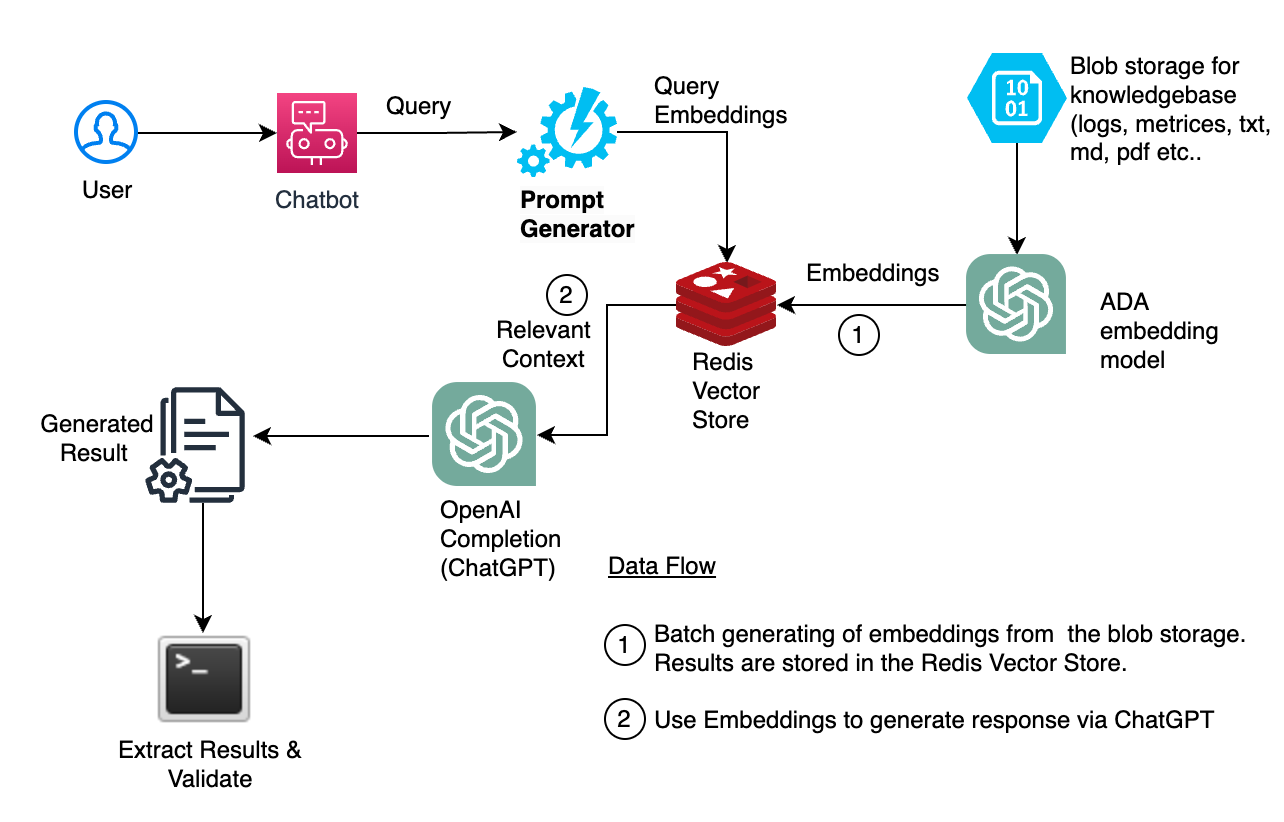
\includegraphics[width=0.8\textwidth]{arch.png}
    \caption{A proposed AIOps framework using LLM-generated results}
    \label{fig:arch}
\end{figure*}

Figure \ref{fig:arch} above shows the proposed implementation of the system. The chatbot can be either UI or API based. In the following subsections, we detail each step of the system more concretely.

\subsection{Log Data}

We use logs from the Apache Zookeeper \cite{zookeeper} application made available on the LogHub GitHub repository \cite{zhu2023loghub}. LogSummary \cite{10017337} also uses the LogHub database. We limit ChatGPT's log input to one grouping of logs, as ChatGPT limits the number of tokens allowed in one prompt inference request. \cite{zhoudb} Listing \ref{lst:zookeeper-example} shows an example of one Zookeeper log group. In the future, it may be possible to perform summarization on longer sequences of logs by performing hierarchical summaries, i.e., summaries of summaries of logs.

We limit the number of groups of Zookeeper logs that we process to 10, as the Azure OpenAI service limits/throttles requests unless we pay a premium.

\begin{figure*}[ht]
\begin{lstlisting}[numbers=none, caption=Zookeeper Log Example, label={lst:zookeeper-example}]
INFO Accepted socket connection from /10.10.34.11 : 49242
WARN Connection request from old client /10.10.34.11 : 49242 ; will be dropped if server is in r-o mode
INFO Client attempting to establish new session at /10.10.34.11 : 49242
INFO Accepted socket connection from /10.10.34.11 : 49244
WARN Connection request from old client /10.10.34.11 : 49244 ; will be dropped if server is in r-o mode
INFO Client attempting to establish new session at /10.10.34.11 : 49244
INFO Established session 0x14ed93111f20037 with negotiated timeout 10000 for client /10.10.34.11 : 49242
INFO Established session 0x14ed93111f20038 with negotiated timeout 10000 for client /10.10.34.11 : 49244
INFO Accepted socket connection from /10.10.34.13 : 37196
WARN Connection request from old client /10.10.34.13 : 37196 ; will be dropped if server is in r-o mode
INFO Client attempting to establish new session at /10.10.34.13 : 37196
INFO Established session 0x14ed93111f20039 with negotiated timeout 10000 for client /10.10.34.13 : 37196
INFO Accepted socket connection from /10.10.34.12 : 45605
WARN Connection request from old client /10.10.34.12 : 45605 ; will be dropped if server is in r-o mode
INFO Client attempting to establish new session at /10.10.34.12 : 45605
INFO Established session 0x14ed93111f2003a with negotiated timeout 10000 for client /10.10.34.12 : 45605
INFO Accepted socket connection from /10.10.34.13 : 37199
WARN Connection request from old client /10.10.34.13 : 37199 ; will be dropped if server is in r-o mode
INFO Client attempting to establish new session at /10.10.34.13 : 37199
INFO Established session 0x14ed93111f2003b with negotiated timeout 10000 for client /10.10.34.13 : 37199
\end{lstlisting}
\end{figure*} 

\subsection{Log Preprocessing}

Presently, we do not have a log preprocessing pipeline set up. We plan to implement a preprocessing pipeline and fill out this section for the project final submission.

% One area that we may find challenging in our research is in the log preprocessing step of the ML pipeline. We would like our proposed system to generalize to various log sources, but logs have a very diverse set of formatting rules and contexts. 

% For example, logs are often found in semi-structured or, in many cases, unstructured formatting. There is no gold standard for logging specifications. Even top companies like Microsoft and Google have had issues with developing a systematic way to standardize logging practices among developers. This lack of log format standardization creates challenges in log parsing. Traditional methods will use regular expressions, keywords, grammar, algorithms, or even statistics to parse and read the logs. \cite{survey-log-aiops}

% Most recent research in the area of log mining and parsing comes from the pre-ChatGPT era. For example, Logram is a library that uses traditional NLP methods such as leveraging n-gram dictionaries to achieve such tasks. \cite{10189040} The method of applying language models to log parsing and mining is still quite new. 

% We may want to consider parsing/preprocessing logs using methods and software proposed previous research. For example, Drain+ \cite{10.1145/3540250.3558947} is a log parser that seeks to address the challenges of six other state-of-the-art log parsers. Drain+ outperforms the other parsers in a study of 16 public datasets.

% Other popular ways of parsing logs include of clustering, pattern mining, and tree-based algorithms. LogMine and LogMa are two popular log parsing libraries that use log clustering with either a K-means algorithm or a hierarchical clustering algorithm. SLCT and LogCluster are two others that look for frequent log file items and perform pattern frequency-based mining. \cite{survey-log-aiops}

% As logs from different applications and systems can be in various formats, it is important that we preprocess the log data to the intended formatting for our application. This means data transformation capabilities are required for our application's data injectors. One popular open-source tool used to ingest and process log data is Logstash, which is compliant with multiple databases/agents such as Telegraf. Alternatively, many proprietary software systems have their own data transformation capabilities that can be used to avoid having additional third-party dependencies. \cite{bendimerad2023onpremise}


\subsection{Knowledgebase - Domain Context Vector Embedding}

The performance of LLMs in log related tasks can be improved by providing the models with more contextual data to use during inference. For example, log data can be used in conjunction with previous incident data to benefit incident management and resolution tasks.

Log data from user input alone may not offer enough insights to produce high-quality generated responses from ChatGPT. Technical documentations, knowledge articles, and/or past incident investigations data can be used to provide contextual information to AIOps tasks, thereby improving task performance. Some examples of these kinds of data include a company's internal root cause knowledge source database, technical documentation of the application or related systems, troubleshooting guides, and software release notes. These data are often unstructured but are beneficial for the generation of analysis and summaries. \cite{saha2022mining}

In our research, we provide the Ada embedding model with a corpus of historical Zookeeper logs and Proxifier logs and corresponding man-made summaries. Ada embeds the tokens found in the corpus and creates a knowledge base consisting of token to vector embedding mappings. By using the Ada embedding model on the historical Zookeeper and Proxifier logs, we obtain a knowledge base that captures the meaning of tokens within the context of Zookeeper and Proxifier logs. We believe this knowledge base can be used to improve the inference prompts we give to ChatGPT. We plan to incorporate this vector search to our prompt for our Prompt Generator in our final milestone 5, as in this milestone 4 we were working on optimizing the search embeddings.

We store the knowledge base vector embeddings in a Redis Vector Store for rapid access during the prompt generation step.

\begin{figure*}[h]
    \centering
    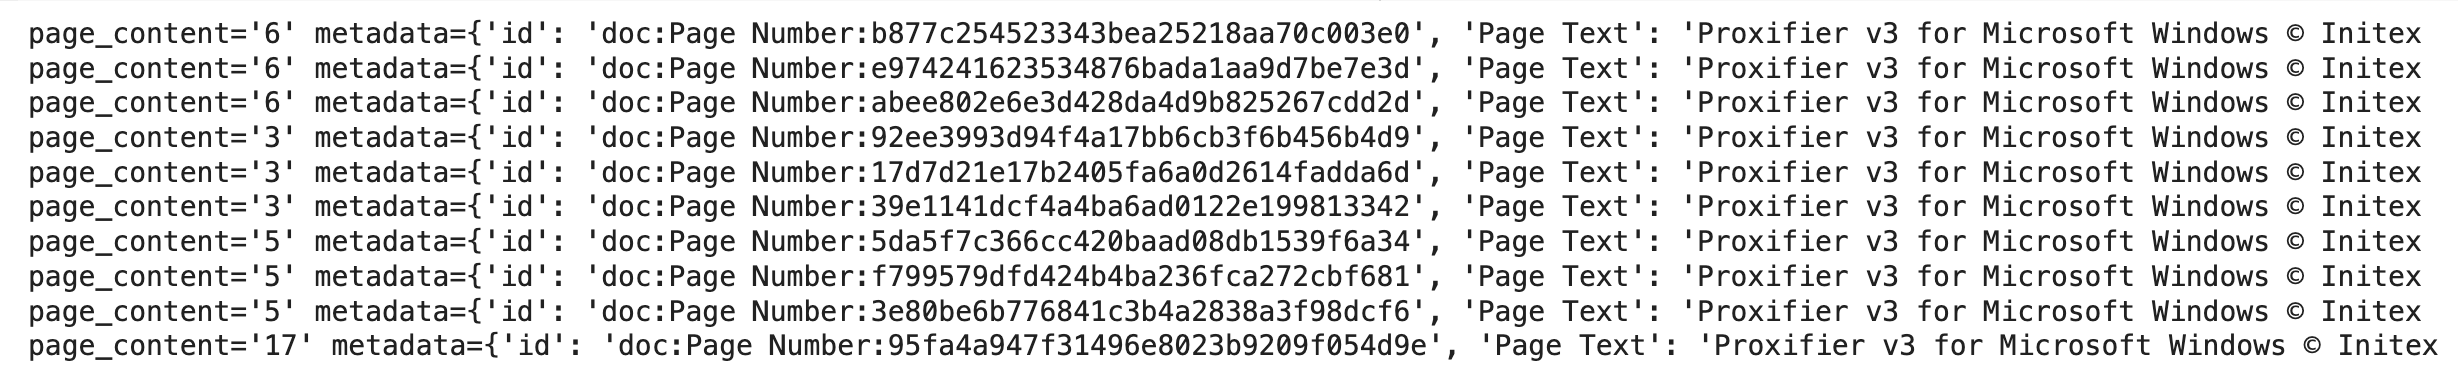
\includegraphics[width=\textwidth]{pagenumber.png}
    \caption{Results with Page Number and Text}
    \label{fig:pagenumber-label}
\end{figure*}

Figure \ref{fig:pagenumber-label} shows the results of using the ADA embedding model to vectorize the contents of the Proxifier documentation. (Note: since we switched to using Zookeeper logs in this milestone, this figure is outdated. This will be updated in the final report).

\subsection{Prompt Engineering}

The performance of chat-based generative LLMs is heavily dependent on the correctness of the input prompts given to the model. When an incorrect or ill-posed prompt given to ChatGPT, ChatGPT is likely to produce a poor output. The prompt needs to be carefully constructed and tuned to generate a specific output that matches user criteria. A well-engineered input prompt can dramatically increase ChatGPT's power to create a good log summary.

In this milestone, we employed a few-shot method which is an important capability of OpenAI's ChatGPT models. The test results shows Few-shot can generate more targeted
and concise summary. In this case, we have generated a json payload which including keys like summary, throughput, and anomaly. Ee can also leverage few-shot to do the processing, for example, we re-format the log files to a more compacted templates by extracting the keywords.

In the next milestone, we will plan take the user-provided prompt that contains the log for which the user would like a summary and append additional contextual information to the prompt before the prompt is sent to ChatGPT for inferencing. We procure the additional contextual information by performing the following steps:


\begin{enumerate}
    \item Extract the log from the user-provided prompt
    \item Embed the log using the same Ada embedding model used to create the logs and summary pair knowledge base
    \item Perform a vector similarity search against the knowledge base vector store
    \item Extract the historical log and associated summary that are similar to the log provided in the prompt, we will pick based on the scores that are returned from the search.
    \item Append the extracted historical log to the prompt
\end{enumerate}

Following these steps, the prompts that will be fed to ChatGPT follow the template shown in Listing \ref{lst:prompt-example}.

\begin{figure*}[ht]
\begin{lstlisting}[numbers=none, caption=Prompt Template Example, label={lst:prompt-example}]
Summarize the following logs from Zookeeper in less than 20 words. The output should be json summary with the keys "summary", "throughput", "anomaly":

<Zookeeper Log>

To help you in this task, the following is a similar log and its associated summary:

Similar Log: <Similar Zookeeper log>
Similar Log Summary: <Similar Zookeeper log summary>
\end{lstlisting}
\end{figure*}

Figure \ref{fig:similar-label} gives an example of computing a similarity score of a given query to the information in the vector store. Similarity score falls in the range [0,1] where 0 indicates dissimilar and 1 indicates nearly identical. In our implementation, which historical contextual log information that is appended to the prompt is determined by selecting the log-log summary pair from the vector store that has the highest similarity score to the log in the input prompt.

\begin{figure} [h]
    \centering
    \includegraphics[width=0.8\linewidth]{Similarity.png}
    \caption{Similarity Scores}
    \label{fig:similar-label}
\end{figure}

\subsection{Models and Inference}

We run embedding and inference using the Azure OpenAI Service API. For embedding and creating the vector store, we use the \lstinline{text-embedding-ada-002} model. We perform log summary generation using the \lstinline{gpt-35-turbo-16k} and \lstinline{gpt-4-32k} ChatGPT models. We generate summaries using both ChatGPT 3.5 and ChatGPT 4 to assess whether ChatGPT 4 performs significantly better than ChatGPT 3.5.

\subsection{Baseline methods}

Presently, we do not implement log summarization with baseline methods. We plan to do so and will fill out this section for the project final submission.

\subsection{Evaluation}

\subsubsection{Vector Store Evaluation}

We employed Redis Vector Store to store our vector embeddings. We utilized the \lstinline{text-embedding-ada-002} model available through the Azure OpenAI service and feed the embeddings with the log and summary Pandas dataframe to the langchain library for vector stores. \cite{ruoccofabrizio}

For embeddings evaluation, the langchain vector store library should run without errors. To ensure that data are stored in Redis, we ran the redis command \lstinline{redis-cli keys "*"} to ensure that the new embeddings are stored in langchain document format. 

Finally, we evaluate the search embeddings performance by feeding a log file that has been fed before, and observe embedding distance of the similarity scores for the returned result. The embedding distance should ideally be close to 0 as lower number means more similar the prediction is to the reference. 

In addition, we try to feed both Proxifier and Zookeeper logs into our Vector Store, and to evaluate that the vector store shoulc not return the search result from the Proxifier logs when we search for Zookeeper logs, or vise versa.

\subsubsection{Summary Generation Evaluation}

Measuring the quality of AI-generated natural language and conversational text is complicated. \cite{wang2023rethinking} To evaluate the quality of the log summaries, we will compute several natural language text generation metrics (see \ref{sec:introduction}). There are two main categories of text generation evaluation metrics: lexical metrics and semantic metrics. Lexical metrics measure the overlap of \textit{vocabulary} between the generated text and a reference text. Semantic metrics measure the similarity of \textit{semantic meaning} between the generated text and a reference text. Semantic metrics are more robust to situations where the generated text is not a 1:1 mapping (e.g., translating a sentence from one natural language to another).

The lexical scores we will compute include BLEU, ROUGE\_L, and METEOR. The semantic scores include BERTScore, BLEURT, and NUBIA.

Our reference text for computing each metric will be the original log that the summary was generated for. In the case of semantic metrics, the metric value is an indication of how much semantic meaning the summary has captured.

\section{Results and Discussion}

\mynote{The results shown in the section are very "work-in-progress" and will change significantly in our final report. So, here we include some draft figures but defer discussion until we have our results finalized.}

\subsubsection{Lexical Scores}

Figures \ref{fig:zookeeper-fewshot-lexical-gpt35}, \ref{fig:zookeeper-fewshot-lexical-gpt4}, \ref{fig:zookeeper-fewshot-lexical-gpt35-gpt4}, \ref{fig:zookeeper-fewshot-lexical-raw-gpt35}, \ref{fig:zookeeper-fewshot-lexical-raw-gpt4}

\begin{figure}[h!]
    \centering
    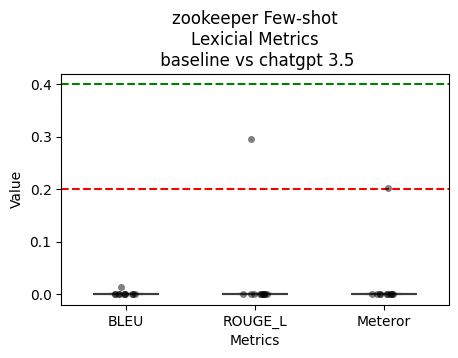
\includegraphics[width=0.5\textwidth]{milestone4/img/zookeeper-few-shot-lexical-3.5.png}
    \caption{ZooKeeper lexical metrics results with few-shot on ChatGPT 3.5}
    \label{fig:zookeeper-fewshot-lexical-gpt35}
\end{figure}

\begin{figure}[h!]
    \centering
    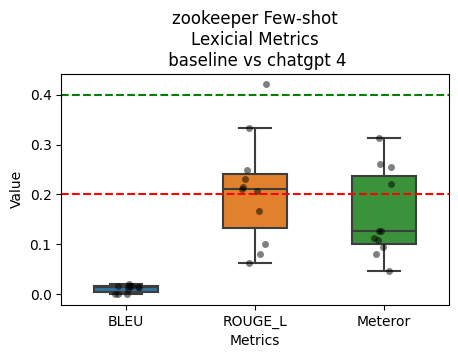
\includegraphics[width=0.5\textwidth]{milestone4/img/zookeeper-few-shot-lexical-4.png}
    \caption{ZooKeeper lexical metrics results with few-shot on ChatGPT 4}
    \label{fig:zookeeper-fewshot-lexical-gpt4}
\end{figure}

\begin{figure}[h!]
    \centering
    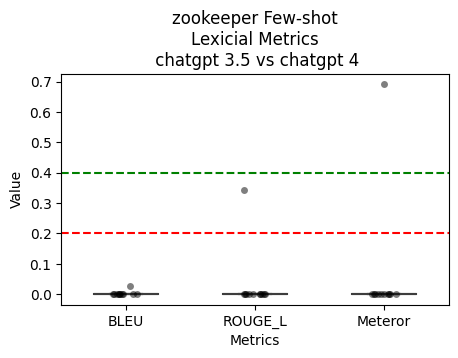
\includegraphics[width=0.5\textwidth]{milestone4/img/zookeeper-few-shot-lexical-35-4.png}
    \caption{ZooKeeper lexical metrics results with few-shot on ChatGPT 3.5 vs ChatGPT 4}
    \label{fig:zookeeper-fewshot-lexical-gpt35-gpt4}
\end{figure}

\begin{figure}[h!]
    \centering
    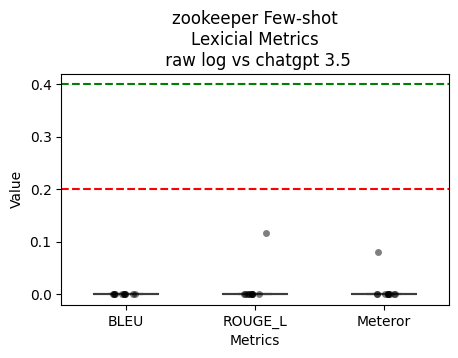
\includegraphics[width=0.5\textwidth]{milestone4/img/zookeeper-few-shot-lexical-raw-35.png}
    \caption{ZooKeeper lexical metrics results with few-shot raw logs vs ChatGPT 3.5}
    \label{fig:zookeeper-fewshot-lexical-raw-gpt35}
\end{figure}

\begin{figure}[h!]
    \centering
    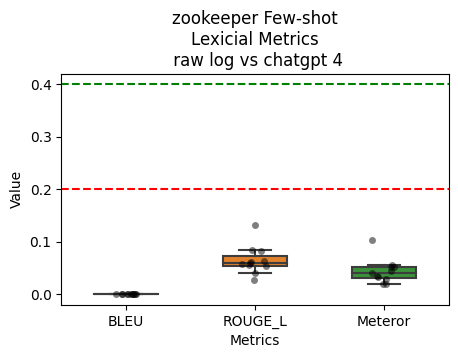
\includegraphics[width=0.5\textwidth]{milestone4/img/zookeeper-few-shot-lexical-raw-4.png}
    \caption{ZooKeeper lexical metrics results with few-shot raw logs vs ChatGPT 4}
    \label{fig:zookeeper-fewshot-lexical-raw-gpt4}
\end{figure}
  
\subsubsection{Semantic Scores}

Figures \ref{fig:zookeeper-fewshot-semantic-gpt35}, \ref{fig:zookeeper-fewshot-semantic-gpt4}, \ref{fig:zookeeper-fewshot-semantic-gpt35-gpt4}, \ref{fig:zookeeper-fewshot-semantic-raw-gpt35}, \ref{fig:zookeeper-fewshot-semantic-raw-gpt4}

\begin{figure}[h!]
    \centering
    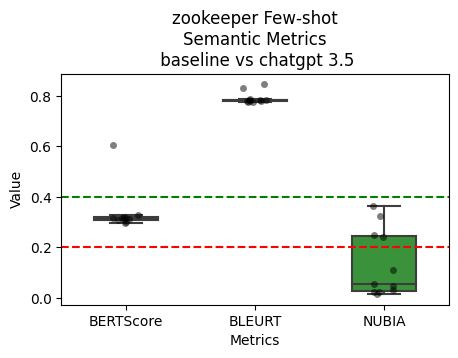
\includegraphics[width=0.5\textwidth]{milestone4/img/zookeeper-few-shot-semantic-3.5.png}
    \caption{ZooKeeper semantic metrics results with few-shot on ChatGPT 3.5}
    \label{fig:zookeeper-fewshot-semantic-gpt35}
\end{figure}

\begin{figure}[h!]
    \centering
    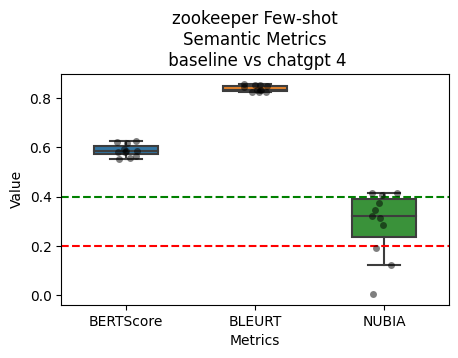
\includegraphics[width=0.5\textwidth]{milestone4/img/zookeeper-few-shot-semantic-4.png}
    \caption{ZooKeeper semantic metrics results with few-shot on ChatGPT 4}
    \label{fig:zookeeper-fewshot-semantic-gpt4}
\end{figure}

\begin{figure}[h!]
    \centering
    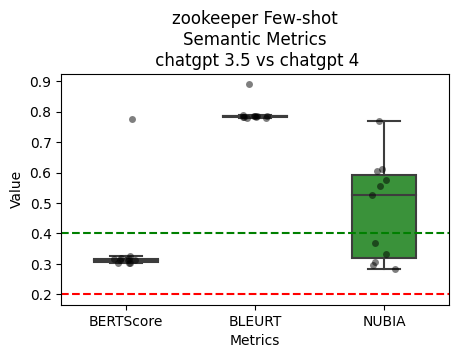
\includegraphics[width=0.5\textwidth]{milestone4/img/zookeeper-few-shot-semantic-35-4.png}
    \caption{ZooKeeper semantic metrics results with few-shot on ChatGPT 3.5 vs ChatGPT 4}
    \label{fig:zookeeper-fewshot-semantic-gpt35-gpt4}
\end{figure}

\begin{figure}[h!]
    \centering
    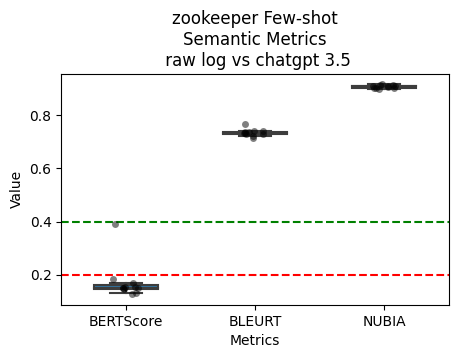
\includegraphics[width=0.5\textwidth]{milestone4/img/zookeeper-few-shot-semantic-raw-35.png}
    \caption{ZooKeeper semantic metrics results with few-shot raw logs vs ChatGPT 3.5}
    \label{fig:zookeeper-fewshot-semantic-raw-gpt35}
\end{figure}

\begin{figure}[ht]
    \centering
    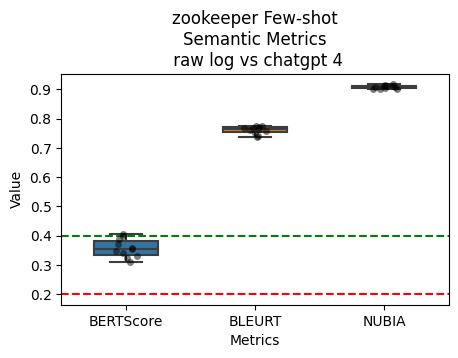
\includegraphics[width=0.5\textwidth]{milestone4/img/zookeeper-few-shot-semantic-raw-4.png}
    \caption{ZooKeeper semantic metrics results with few-shot raw logs vs ChatGPT 4}
    \label{fig:zookeeper-fewshot-semantic-raw-gpt4}
\end{figure}

\subsubsection{Vector Store}

Figures \ref{fig:redis-cli}, \ref{fig:redis-proxifier}, \ref{fig:redis-zookeeper}

\begin{figure}
    \centering
    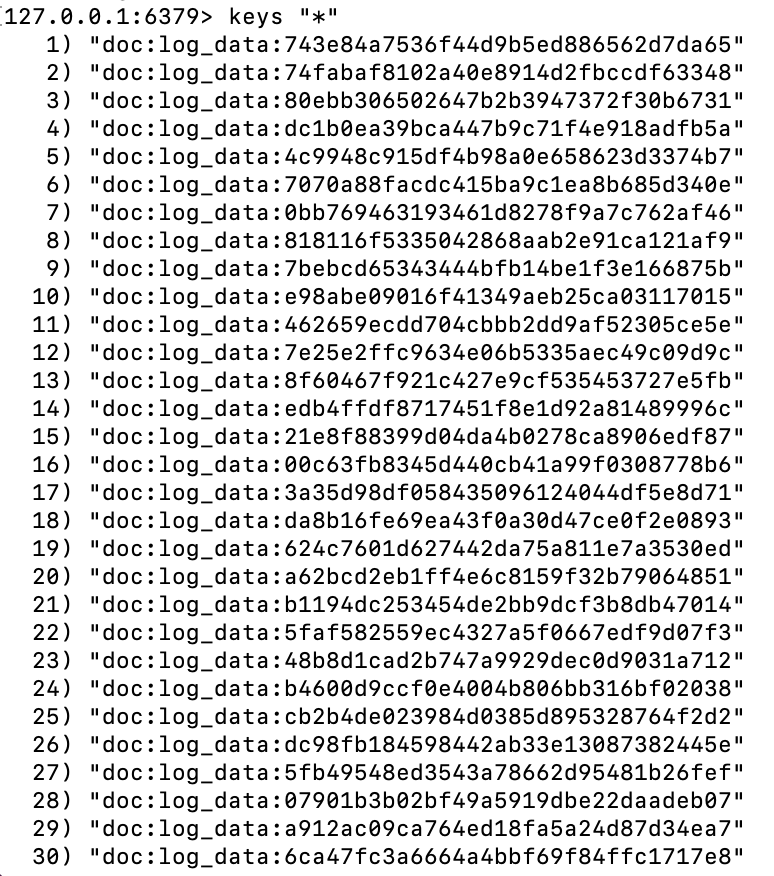
\includegraphics[width=0.7\linewidth]{Screen Shot 2023-11-19 at 8.35.39 PM.png}
    \caption{Validated the output from redis-cli to ensure that the embeddings are stored successfully}
    \label{fig:redis-cli}
\end{figure}

\begin{figure}
    \centering
    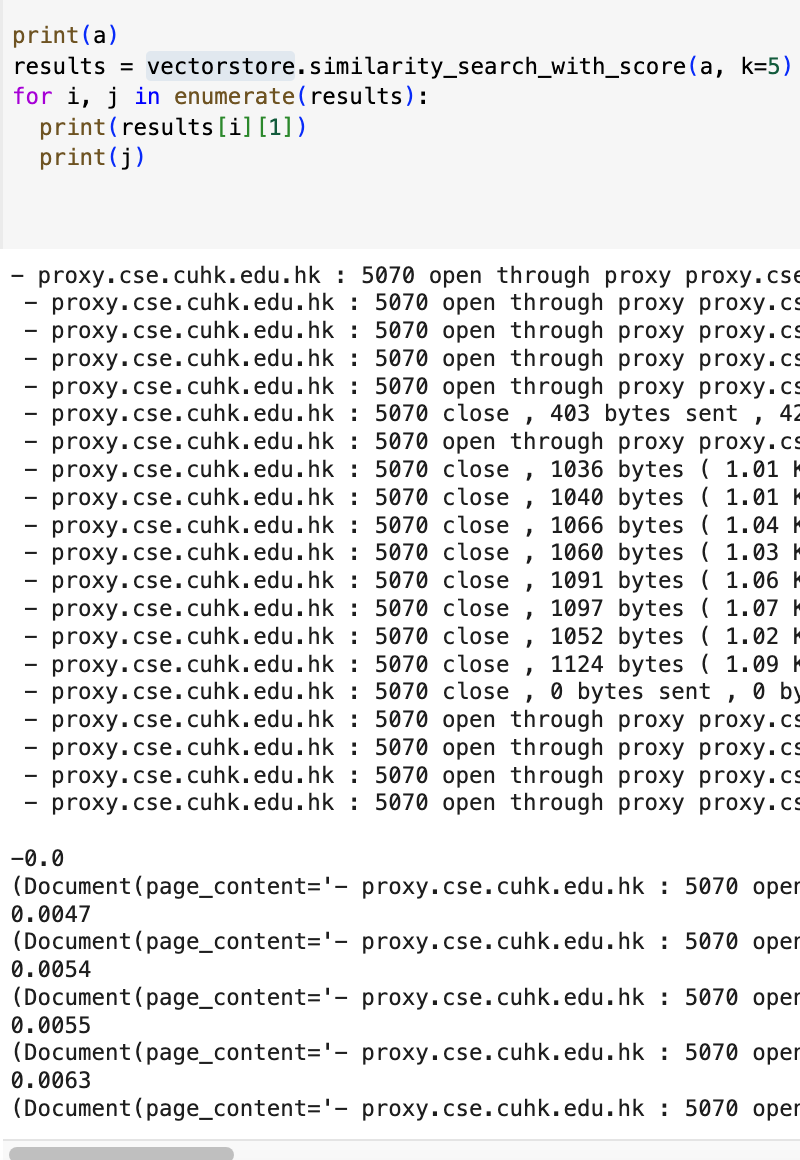
\includegraphics[width=0.7\linewidth]{Screen Shot 2023-11-19 at 9.00.20 PM.png}
    \caption{Validated the output from vector store that the embedding distance is close to 0 for a Proxifier log search that existed in the vector store, and to ensure that the results returned belongs to Proxifier logs.}
    \label{fig:redis-proxifier}
\end{figure}

\begin{figure}
    \centering
    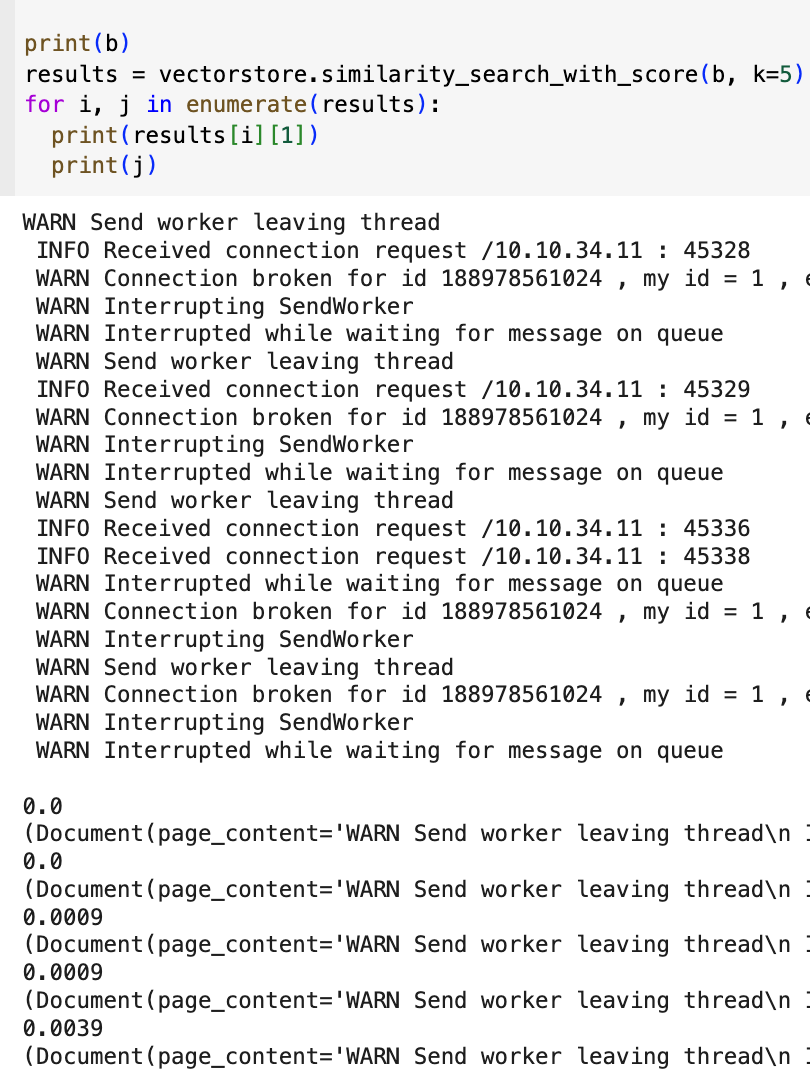
\includegraphics[width=0.8\linewidth]{Screen Shot 2023-11-19 at 9.03.00 PM.png}
    \caption{Validated the output from vector store that the embedding distance is close to 0 for a Zookeeper log search that existed in the vector store, and to ensure that the results returned belongs to Zookeeper logs.}
    \label{fig:redis-zookeeper}
\end{figure}

\subsection{Ablations}

This section will be filled out in the final submission. We plan to perform an ablation study in which we omit the step of appending contextual information to the prompt before sending the prompt to ChatGPT.

\section{Conclusion}

\mynote{This section is copied from milestone 3 and will be updated in our final report to better reflect the results we obtain in our research.}

Overall, we believe that our system is going to benefit companies of all sizes and improve their IT Operations workflows in a modern complex cloud infrastructure, as they often are unable to allocate the necessary resources and budget to train and fine-tune large ML models. We expect the following stakeholders to benefit from this project:
\begin{itemize}
    \item Site Reliability Engineers
    \item Platform Engineers 
    \item Management Audience 
    \item Incident Commanders 
\end{itemize}

We expect that SREs and Platform Engineers are the stakeholders that will benefit the most as our framework can used as an assistance tool for SREs when when maintaining cloud systems or responding to cloud incidents. Managers can use this tool to understand the current situation of the infrastructure without knowing many technical details. The incident commander can use this tool to ensure that the analysis is flowing in the right direction. Finally, we believe now is an optimal time to incorporate Generative AI into the corporate world within the IT Operations field. We hope this framework can transform how incident management, alerting, and root cause analysis are performed. 

\bibliographystyle{plain}
\bibliography{ref}
\vspace{12pt}

\end{document}